\documentclass[singlesided,
  paper=a4,
  fontsize=10pt
]{resume}

% Set geometry
% ------------------------------------------------------------------------------
\setlength\highlightwidth{6.5cm}
% Note that margintop gets added to this value, i.e. the header bar is 5cm
\setlength\headerheight{3cm}
\setlength\marginleft{0.5cm}
\setlength\marginright{\marginleft}
\setlength\margintop{1cm}
\setlength\marginbottom{1cm}

% IMAGES PATH
% ------------------------------------------------------------------------------
\graphicspath{ {../img/} }

% FONTS
% ------------------------------------------------------------------------------
\setmainfont{\custommainfont}
\renewfontfamily\nerdfont{\customnerdfont}

% COLORS
% ------------------------------------------------------------------------------

% Content
% ------------------------------------------------------------------------------
\begin{document}
\name{Romain Deville}
\tagline{%
Passioné par l'informatique, je me suis spécialisé dans l'administration
système et plus particulièrement l'automatisation de déploiement et de
provisionnement.\\ J'attache aussi beaucoup d'importance à mes investissements
associatifs ainsi qu'à la protection des données privées.
}
% Make photo exactly match the header with margintop/marginright/marginbottom
% as margin
\photo[square]{logo_rdeville.png}{\dimexpr \headerheight-\marginbottom}
\makeheader

\highlightbar{
  \section[\nerdfont]{Contact}
    \email{pro@romaindeville.fr}
    \phone{+33.6.70.80.04.88}
    \location{%
      15 rue Philippe Lebon \newline
      52110
      Dommartin le Franc \newline
      France
    }
    \driver{Permis B}
  \section[\nerdfont]{Network}
    \homepage{https://romaindeville.fr}
    \profile%
      {Book-Reader}%
      {https://docs.romaindeville.fr}%
      {https://docs.romaindeville.fr}%
      {Documentation de mes projets}
    \profile%
      {Gitlab}%
      {http://framagit.com/rdeville.public}%
      {@rdeville}%
      {}
    \profile%
      {Github}%
      {http://github.com/rdeville}%
      {@rdeville}%
      {}
    \profile%
      {Docker}%
      {https://hub.docker.com/u/rdeville}%
      {rdeville}%
      {}
    \profile%
      {LinkedIn}%
      {https://www.linkedin.com/in/romaindeville}%
      {Romain Deville}%
      {}
  \section[\fa{language}]{Languages}
    \lang%
      {Français}%
      {100}%
      {
\includegraphics[height=1em,width=2em]{flag/francais.png}}%
      {Langue Natale}%
      {green_800}
    \lang%
      {Anglais}%
      {90}%
      {
\includegraphics[height=1em,width=2em]{flag/anglais.png}}%
      {Courant}%
      {green_800}
  \section[\nerdfont]{Skills}
    \skillsection{Programmation}
      \skill%
        {Bash/Shell}%
        {95}%
        {
\includegraphics[height=1em]{skill/bash.png}}%
        {}%
        {indigo_800}
      \skill%
        {Python}%
        {80}%
        {
\includegraphics[height=1em]{skill/python.png}}%
        {}%
        {indigo_800}
      \skill%
        {HTML/CSS}%
        {60}%
        {
\includegraphics[height=1em]{skill/html_css.png}}%
        {}%
        {indigo_800}
      \skill%
        {LaTeX}%
        {90}%
        {
\includegraphics[height=1em]{skill/latex.png}}%
        {}%
        {indigo_800}
      \skill%
        {C++}%
        {50}%
        {
\includegraphics[height=1em]{skill/cpp.png}}%
        {}%
        {indigo_800}
    \skillsection{Système d'Exploitation}
      \skill%
        {Linux}%
        {90}%
        {
\includegraphics[height=1em]{skill/linux.png}}%
        {(e.g. Ubuntu, Debian, Arch, Centos, ...)}%
        {blue_800}
      \skill%
        {MacOS}%
        {80}%
        {
\includegraphics[height=1em]{skill/apple.png}}%
        {}%
        {blue_800}
      \skill%
        {Windows}%
        {80}%
        {
\includegraphics[height=1em]{skill/windows.png}}%
        {}%
        {blue_800}
    \skillsection{Logiciel et Outils}
      \skill%
        {Ansible}%
        {90}%
        {
\includegraphics[height=1em]{skill/ansible.png}}%
        {}%
        {light_blue_800}
      \skill%
        {Docker}%
        {60}%
        {
\includegraphics[height=1em]{skill/docker.png}}%
        {}%
        {light_blue_800}
      \skill%
        {Kubernetes}%
        {60}%
        {
\includegraphics[height=1em]{skill/kubernetes.png}}%
        {}%
        {light_blue_800}
      \skill%
        {OpenStack}%
        {80}%
        {
\includegraphics[height=1em]{skill/openstack.png}}%
        {}%
        {light_blue_800}
      \skill%
        {Monitoring}%
        {70}%
        {
\includegraphics[height=1em]{skill/monitoring.png}}%
        {(e.g. Prometheus, Grafana, ELK, ...)}%
        {light_blue_800}
      \skill%
        {Office}%
        {90}%
        {
\includegraphics[height=1em]{skill/office.png}}%
        {(e.g. LibreOffice, MS Office, ...)}%
        {light_blue_800}
      \skill%
        {Graphisme}%
        {60}%
        {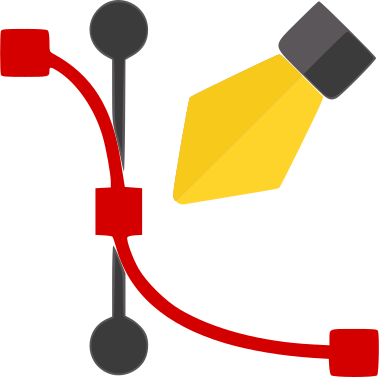
\includegraphics[height=1em]{skill/graphism.png}}%
        {(e.g. Gimp, Inkscape, Adobe Suite, ...)}%
        {light_blue_800}
}

\mainbar{
  \section[\fa{cogs}]{Work Experiences}%
    \vspace{-1em}
    \jobcompany%
      {work/liris.png}%
      {LIRIS}%
      {https://liris.cnrs.fr}%
      {Villeurbanne, Rhone-Alpes, France}%
      {}%
    \jobposition%
      {Ingénieur d'Etudes}%
      {Sep 2018\textendash Aug 2020}%
      {2 years}%
      {
Mise en place d'outils pour le deployement d'une plateforme de calcul
scientifique permettant la reproductibilité des resultats.}
      {%
        \begin{itemize}
          \item Conception \& Développement
          \item Diriger l'équipe de soutien.
        \end{itemize}
      }%
        \textcolor{midrules}{\rule{\linewidth}{0.5pt}}
    \jobposition%
      {Doctorant}%
      {Sep 2014\textendash Aug 2018}%
      {4 years}%
      {
Projet de recherche ayant pour but de développer de nouveaux modèles et outils
pour représenter des données 2D (images) et 2D+t (vidéos, automate
cellulaire). Projet ANR SoLSTiCe.}
      {%
        \begin{itemize}
          \item Développement d'outils et d'algorithme de fouille
          \item Plannification des expérimentations
          \item Travail en autonomie
        \end{itemize}
      }%
        \textcolor{midrules}{\rule{\linewidth}{0.5pt}}
    \jobposition%
      {Stagiaire}%
      {Jun 2011\textendash Aug 2011}%
      { 3 months}%
      {
Développement d'un outils de visualisation et de modélisation Web 3D d'un
bâtiment intelligent avec la possibilité d'effectuer des requêtes sur des
capteurs.}
      {}%
  \section[\fa{hands-helping}]{Volunteer Experiences}
    \volunteerorganization%
      {association/lov.png}%
      {LOV}%
      {https://labovilleurbanne.fr/site/}%
      {FabLab - Laboratoire Ouvert Villeurbannais}%
      {Villeurbanne, Rhone-Alpes, France}%
      {
        \volunteerposition%
          {Membre du CA}%
          {Jun 2019\textendash Jun 2020}%
          {1 year}%
          {}
        \volunteerposition%
          {Membre Actif}%
          {Jun 2018\textendash Nov 2020}%
          {2 years 5 months}%
          {}
      }
      \hspace{0.01\linewidth}{\color{midrules}\vline}\hfill
    \volunteerorganization%
      {association/illyse.png}%
      {Illyse}%
      {https://www.illyse.net}%
      {Fournisseur d'Accès Associatif à Lyon et Saint-Etienne}%
      {Lyon, Rhone-Alpes, France}%
      {
        \volunteerposition%
          {Membre du CA}%
          {Mar 2017\textendash Nov 2020}%
          {3 years 8 months}%
          {}
        \volunteerposition%
          {Membre Actif}%
          {Mar 2016\textendash Nov 2020}%
          {4 years 8 months}%
          {}
      }
      \textcolor{midrules}{\rule{\linewidth}{0.5pt}}%
      \vspace{-1em}
    \volunteerorganization%
      {association/mpt.jpg}%
      {Salle des Rancy}%
      {https://www.salledesrancy.com/}%
      {MJC, Maison Pour Tous - Salle des Rancy}%
      {Lyon, Rhone-Alpes, France}%
      {
        \volunteerposition%
          {Bénévole}%
          {Jun 2016\textendash Nov 2020}%
          {4 years 5 months}%
          {}
      }
      \hspace{0.01\linewidth}{\color{midrules}\vline}\hfill
    \volunteerorganization%
      {association/grainesdimages.png}%
      {Graines d'Images}%
      {https://www.grainesdimages.fr/}%
      {Association de photographie de l'INSA de Lyon}%
      {Villeurbanne, Rhone-Alpes, France}%
      {
        \volunteerposition%
          {Membre Actif}%
          {Jun 2009\textendash Jun 2018}%
          {9 years}%
          {}
        \volunteerposition%
          {Vice-Président}%
          {Jun 2010\textendash Jun 2011}%
          {1 year}%
          {}
        \volunteerposition%
          {Trésorier}%
          {Jun 2012\textendash Jun 2013}%
          {1 year}%
          {}
      }
  \vspace{-1.5em}
  \section[\fa{graduation-cap}]{Education}
    \schooldiploma
      {Doctorat en Informatique de l'université de Lyon opéré à l'INSA de Lyon}
      {2014\textendash 2018}
      {Villeurbanne, Rhone-Alpes, France}
      {Institut National des Sciences Appliquées de Lyon (INSA)}
      {https://www.insa-lyon.fr/}
      {
Fouille de grilles en 2D et 2D+t appliquée à la classification d'images et
l'analyse d'automate cellulaires.}
    \textcolor{lightgray}{\rule{\linewidth}{0.25pt}}
    \schooldiploma
      {Diplome d'Ingénieur, Spécialité Informatique}
      {2010\textendash 2014}
      {Villeurbanne, Rhone-Alpes, France}
      {Institut National des Sciences Appliquées de Lyon (INSA)}
      {https://www.insa-lyon.fr/}
      {
Développement, intégration logiciel, systèmes et réseaux, informatique
décisionnelle, systèmes d'information, gestion de projet, management.}
    \textcolor{lightgray}{\rule{\linewidth}{0.25pt}}
    \schooldiploma
      {Classe Préparatoire Intégrée}
      {2008\textendash 2010}
      {Villeurbanne, Rhone-Alpes, France}
      {Institut National des Sciences Appliquées de Lyon (INSA)}
      {https://www.insa-lyon.fr/}
      {
$2^{nd}$ année en Section international (SCAN)}
    \textcolor{lightgray}{\rule{\linewidth}{0.25pt}}
    \schooldiploma
      {Baccalauréat Scientifique SVT, Spécialité Mathématique}
      {2005\textendash 2008}
      {Chaumont, Haute-Marne, France}
      {Lycée Charles de Gaulle}
      {}
      {
Mention Bien, Mention Européenne}
  \section[\nerdfont]{Interests}
  \interest%
    {Photographie}%
    {Pratique de la photographie argentique, numérique et polaroid.}
    {\nerdfont}
  \interest%
    {Vélo}%
    {Principal moyen de transport, j'aime aussi personaliser mon vélo.}
    {\nerdfont}
  \interest%
    {Auto-Hébergement}%
    {J'heberge mes propres mails et mon stockage en ligne depuis 2016.}
    {\nerdfont}
  \interest%
    {Do It Yourself (DIY)}%
    {J'heberge mes propres mails et mon stockage en ligne depuis 2016.}
    {\nerdfont}
}
\makebody

\end{document}
% *****************************************************************************
% VIM MODELINE
% vim: ft=tex
% *****************************************************************************